
%(BEGIN_QUESTION)
% Copyright 2006, Tony R. Kuphaldt, released under the Creative Commons Attribution License (v 1.0)
% This means you may do almost anything with this work of mine, so long as you give me proper credit

A pressure-relief valve installed in a hydraulic system acts sort of like a {\it shunt voltage regulator} circuit: it limits pressure by bypassing (shunting) fluid back to the reservoir.

$$\includegraphics[width=15.5cm]{i00759x01.eps}$$

Qualitatively determine what will happen to the pressure-relief valve's return flow rate (back to the reservoir) for each of the following conditions, and be prepared to explain {\it why} for each case.  Consider each condition as an independent event, without reference to previous conditions:

\begin{itemize}
\item{} Hand lever is moved from the ``stop'' position to the ``run'' position ; return flow ({\it increases}, {\it decreases}, or {\it stays the same})?
\item{} Hand lever is moved from the ``run'' position to the ``stop'' position ; return flow ({\it increases}, {\it decreases}, or {\it stays the same})?
\item{} While running, the hydraulic motor encounters a heavier mechanical load ; return flow ({\it increases}, {\it decreases}, or {\it stays the same})? 
\item{} With the hydraulic motor stopped, the pump speed is decreased ; return flow ({\it increases}, {\it decreases}, or {\it stays the same})? 
\end{itemize}

\underbar{file i00759}
%(END_QUESTION)





%(BEGIN_ANSWER)

\begin{itemize}
\item{} Hand lever is moved from the ``stop'' position to the ``run'' position ; return flow {\bf decreases}.
\item{} Hand lever is moved from the ``run'' position to the ``stop'' position ; return flow {\bf increases}.
\item{} While running, the hydraulic motor encounters a heavier mechanical load ; return flow {\bf increases}, but only if the pressure has risen to its maximum value.  Otherwise, the return flow will {\bf stay the same} at zero. 
\item{} With the hydraulic motor stopped, the pump speed is decreased ; return flow {\bf decreases}.
\end{itemize}

%(END_ANSWER)





%(BEGIN_NOTES)

\vfil \eject

\noindent
{\bf Summary Quiz:}

Predict the effect of the spring breaking inside the pressure relief valve, so that it no longer exerts a force against the internal valve mechanism:

$$\includegraphics[width=15.5cm]{i00759x01.eps}$$

\begin{itemize}
\item{} The hydraulic motor will reverse direction
\vskip 5pt 
\item{} The hydraulic pump's speed will decrease slightly
\vskip 5pt 
\item{} The hydraulic motor will become very ``weak'' (lose power) 
\vskip 5pt 
\item{} The hand-actuated lever will become difficult to move
\vskip 5pt 
\item{} The oil reservoir will eventually run empty 
\vskip 5pt 
\item{} The hydraulic pump will stall (``lock up'' and refuse to turn)
\end{itemize}


%INDEX% Mechanics, fluid power systems: pressure relief valve flow rate

%(END_NOTES)


